% !TeX root = ../tfg.tex
% !TeX encoding = utf8

\chapter{Técnicas de Deep Learning} \label{chap:dl-info}

En este capítulo se describen las principales estrategias probadas de deep learning para abordar el problema de la predicción de complicaciones en biopsias pulmonares a partir de datos de tomografía computarizada. Se presentan tanto los enfoques iniciales basados en cortes bidimensionales (2D) como la evolución hacia modelos tridimensionales (3D) que aprovechan de forma completa la información volumétrica de las imágenes.  

\section{Enfoque basado en cortes 2D}

En las fases iniciales del proyecto se planteó abordar el problema utilizando modelos convolucionales 2D entrenados sobre cortes axiales extraídos de los volúmenes de TC. Se empezó por esta técnica ya que computacionalmente conllevaba menos requisitos. Esto se debe a que los modelos 2D son más ligeros, rápidos de entrenar y pueden aprovechar pesos preentrenados en tareas de visión convencional.

El procedimiento consistía en dividir cada volumen 3D en múltiples cortes axiales, que se preprocesaban de forma individual para usarse como muestras independientes durante el entrenamiento. El objetivo era que el modelo aprendiera a clasificar cada corte según la presencia o ausencia de complicaciones. Sin embargo, esto planteaba varios desafíos importantes: por un lado, la predicción debía agregarse finalmente a nivel de paciente, no de corte aislado; por otro, al tratarse de volúmenes reales, muchas de las slices correspondían a regiones extremas sin tejido pulmonar visible, lo que introducía información confusa y dificultaba el aprendizaje efectivo del modelo.

Otras de las limitaciones de este enfoque es que al trabajar con slices individuales, se pierde la información espacial tridimensional presente en el volumen completo. La relación entre cortes consecutivos, que puede contener patrones anatómicos relevantes para predecir complicaciones, queda ignorada. Además, la variabilidad en el número de cortes entre pacientes complica la agregación de predicciones y la estandarización.

Debido a estos factores, y especialmente a los malos resultados obtenidos en las primeras pruebas, se decidió descartar rápidamente esta aproximación en favor de un enfoque 3D para aprovechar la naturaleza de los datos.


\subsection{Descripción de las arquitecturas empleadas 2D}

\subsubsection{EfficientNetV2}
EfficientNetV2  \parencite{tan2021efficientnetv2} es una familia de redes neuronales convolucionales diseñadas para ser especialmente eficientes en términos de velocidad de entrenamiento y uso de recursos computacionales. Su principal objetivo es lograr un buen equilibrio entre precisión, tamaño del modelo y tiempo de entrenamiento, aspectos especialmente importantes cuando se dispone de recursos limitados o se buscan aplicaciones prácticas en entornos clínicos.

A diferencia de modelos anteriores más pesados, EfficientNetV2 introduce mejoras en la forma en que se organiza y escala la arquitectura. En lugar de simplemente hacer la red más profunda o ancha de manera uniforme, aplica un \textit{escalado compuesto} más inteligente, que distribuye la complejidad donde más se necesita. Esto significa que se añaden capas de forma más selectiva en determinadas etapas de la red, optimizando el uso de parámetros y reduciendo el tiempo de entrenamiento sin sacrificar precisión.

Además, este modelo introduce bloques de convolución más simples y rápidos, llamados \textit{Fused-MBConv}, que combinan de forma eficiente operaciones convolucionales para reducir la sobrecarga de memoria y acelerar el entrenamiento. La estructura de estos bloques está representada en la Figura \ref{fig:efficientnetv2}. Esta simplificación permite entrenar modelos de buena capacidad en menos tiempo.

En este proyecto se utilizó la variante \texttt{EfficientNetV2-S}, una configuración compacta y rápida, pensada para ofrecer un rendimiento competitivo sin alzar mucho el coste computacional. Es por eso por lo que hemos elegido esta red frente a otras, ya que resulta adecuada para trabajar con imágenes 2D de cortes axiales, donde la eficiencia es clave para poder procesar grandes volúmenes de datos en tiempos razonables.

\begin{figure}[!htbp]
    \centering
    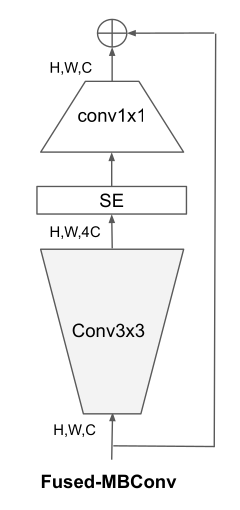
\includegraphics[width=0.25\textwidth]{img/efficientnetv2.png}
    \caption{Estructura de Fused-MBConv \parencite{tan2021efficientnetv2}.}
    \label{fig:efficientnetv2}
\end{figure}


\section{Enfoque basado en volúmenes 3D}

Dada la naturaleza volumétrica de los datos de TC, un enfoque más adecuado consiste en procesar directamente el volumen tridimensional completo. Para ello, utilizamos redes neuronales convolucionales 3D que extienden las operaciones de convolución y pooling clásicas a tres dimensiones, trabajando sobre la altura, anchura y profundidad (número de slices).

En general, muchas arquitecturas 2D pueden adaptarse a 3D de forma relativamente directa, sustituyendo las capas de convolución 2D por convoluciones 3D (con kernels típicos de $3 \times 3 \times 3$) y aplicando pooling 3D. Esto permite a la red capturar patrones espaciales en las tres dimensiones. Las dos arquitecturas empleadas en este trabajo, \textit{ResNet} y \textit{DenseNet} han sido adaptadas a este formato, manteniendo la esencia de sus diseños originales pero generalizando sus operaciones al espacio tridimensional.

Un aspecto importante para trabajar con volúmenes 3D es la necesidad de normalizar el tamaño de entrada. Los volúmenes originales, como vimos en la sección \ref{eda} presentan variabilidad en el número de slices y resolución axial (512x512 o 768x768). En la propia sección, en el preprocesamiento, se realizó interpolación trilineal para estandarizar todos los volúmenes a un tamaño (se realizaron múltiples interpolaciones para poder probar diferentes tamaños). Esto es esencial para permitir el procesamiento en batch y la compatibilidad con arquitecturas convolucionales profundas.

\subsection{Procedimiento general de entrenamiento}

El procedimiento seguido es muy común en aprendizaje profundo pero con adaptaciones necesarias para trabajar con imágenes médicas volumétricas y un dataset relativamente pequeño.

En primer lugar, se define la arquitectura del modelo. En este trabajo se utilizó principalmente DenseNet121 adaptado a 3D, una arquitectura que incluye bloques densos con conexiones entre todas las capas, lo que mejora la propagación de gradientes y favorece la reutilización de características. 

Durante el entrenamiento, se emplea un enfoque supervisado clásico, utilizando la \textit{CrossEntropyLoss} como función de pérdida para la tarea de clasificación binaria (complicación sí/no). El optimizador más usado fue \textit{Adam}, conocido por ser efectivo con datos heterogéneos y tamaños de batch reducidos. En algunas configuraciones, se experimentó con \textit{weight decay} para ayudar a evitar el sobreajuste.

Para cada fold, se entrena el modelo durante varias épocas monitorizando métricas clave en el conjunto de validación, como accuracy, F1-score o G-Mean, para identificar el modelo con mejor desempeño. Además, se aplican técnicas como \textit{early stopping} y ajustes de regularización como dropout para mitigar el sobreajuste dada la limitada cantidad de datos.

Adicionalmente, se aplicaron técnicas de explicabilidad como Grad-CAM o Shap para analizar las regiones de los volúmenes en las que el modelo basaba sus decisiones, asegurando así que el aprendizaje se centraba en el tejido pulmonar relevante y no en artefactos o regiones externas. 

En resumen, el entrenamiento de los modelos se diseñó de forma modular con optimización, regularización y validación, adaptadas al nuestro problema específico con datos 3D limitados.



\subsection{Descripción de las arquitecturas empleadas 3D}
Durante toda la fase de implementación se han probado varios modelos. Los dos principales son ResNet3D y DenseNet121 3D. 

\subsubsection{Resnet}
Las 3D ResNets (Residual Networks) son una extensión natural de las ResNets 2D al dominio volumétrico \parencite{hara2017learning}. Conservan la idea clave de las \textit{conexiones de salto} (skip connections), que ayudan a mitigar el problema del gradiente desvanecido al permitir un flujo de información más directo entre capas distantes.  

En su adaptación 3D, tanto las convoluciones como las operaciones de pooling se aplican en las tres dimensiones espaciales. Por ejemplo, se utilizan kernels convolucionales de $3 \times 3 \times 3$, y el downsampling se realiza con stride 2 en todas las dimensiones. Esto permite a la red capturar contextos espaciales tridimensionales completos, cruciales en tareas como la segmentación o la predicción de riesgos en TC. Su arquitectura se puede observar en la Tabla \ref{tab:resnet_arch}.

Las 3D ResNets han demostrado ser más precisas que arquitecturas más simples, especialmente cuando se dispone de suficiente capacidad de cómputo y datos bien preprocesados.


\begin{table}[!htbp]
\centering
\caption{Arquitectura ResNet 3D. Los bloques residuales se muestran entre paréntesis. Cada capa convolucional va seguida de normalización por lotes y ReLU. El muestreo descendente se realiza mediante conv3\_1, conv4\_1, conv5\_1 con un paso de 2. La dimensión de la última capa totalmente conectada se establece para el conjunto de datos Kinetics (400 categorías) \parencite{hara2017learning}.}
\label{tab:resnet_arch}
\begin{tabular}{ccc}
\hline
Nombre de la capa & Arquitectura (18-layer) & Arquitectura (34-layer) \\
\hline
conv1 & $7 \times 7 \times 7$, 64, stride 1 (T), 2 (XY) & \\
\hline
conv2\_x & 3 $\times$ 3 $\times$ 3 max pool, stride 2 &  \\
         & $\left[\begin{array}{c}
         3 \times 3 \times 3, 64 \\
         3 \times 3 \times 3, 64
         \end{array}\right] \times 2$ &
         $\left[\begin{array}{c}
         3 \times 3 \times 3, 64 \\
         3 \times 3 \times 3, 64
         \end{array}\right] \times 3$ \\
\hline
conv3\_x & $\left[\begin{array}{c}
         3 \times 3 \times 3, 128 \\
         3 \times 3 \times 3, 128
         \end{array}\right] \times 2$ &
         $\left[\begin{array}{c}
         3 \times 3 \times 3, 128 \\
         3 \times 3 \times 3, 128
         \end{array}\right] \times 4$ \\
\hline
conv4\_x & $\left[\begin{array}{c}
         3 \times 3 \times 3, 256 \\
         3 \times 3 \times 3, 256
         \end{array}\right] \times 2$ &
         $\left[\begin{array}{c}
         3 \times 3 \times 3, 256 \\
         3 \times 3 \times 3, 256
         \end{array}\right] \times 6$ \\
\hline
conv5\_x & $\left[\begin{array}{c}
         3 \times 3 \times 3, 512 \\
         3 \times 3 \times 3, 512
         \end{array}\right] \times 2$ &
         $\left[\begin{array}{c}
         3 \times 3 \times 3, 512 \\
         3 \times 3 \times 3, 512
         \end{array}\right] \times 3$ \\
\hline
\multicolumn{3}{c}{average pool, 400-d fc, softmax} \\
\hline
\end{tabular}
\end{table}




\subsubsection{Arquitectura DenseNet-121}

DenseNet (Densely Connected Convolutional Network) propone un esquema de conectividad densa en el que cada capa recibe como entrada todos los mapas de características de las capas anteriores, favoreciendo la reutilización de características y mejorando el flujo de gradientes \parencite{huang2017densely}. Esta idea también puede extenderse de forma natural al dominio tridimensional. Véase Figuras \ref{fig:densenet2} y \ref{fig:densenet1}.

En la versión 3D de DenseNet-121, todas las convoluciones 2D se sustituyen por convoluciones 3D, manteniendo la estructura en bloques densos y capas de transición con pooling 3D. Este diseño permite capturar patrones volumétricos complejos y facilita el aprendizaje de representaciones más expresivas con menos parámetros, aprovechando la reutilización de características intermedias.  

Una característica importante es la inclusión de capas bottleneck (convoluciones 1x1x1) que reducen el número de canales de entrada, esto simplifica el modelo sin alterar la resolución espacial, antes de aplicar convoluciones más costosas de 3x3x3. Además, se emplean capas de transición con average pooling para reducir progresivamente la resolución espacial del volumen.

\begin{figure}[!htbp]
    \centering
    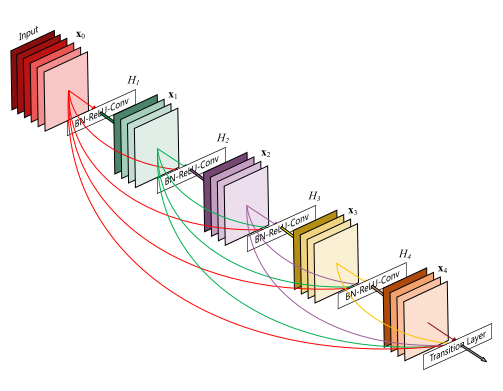
\includegraphics[width=0.7\textwidth]{img/densenet121_2.png}
    \caption{Un bloque denso de 5 capas con una tasa de crecimiento de $k=4$. Cada capa toma como entrada todos los mapas de características anteriores \parencite{huang2017densely}.}
    \label{fig:densenet2}
\end{figure}


\begin{figure}[!htbp]
    \centering
    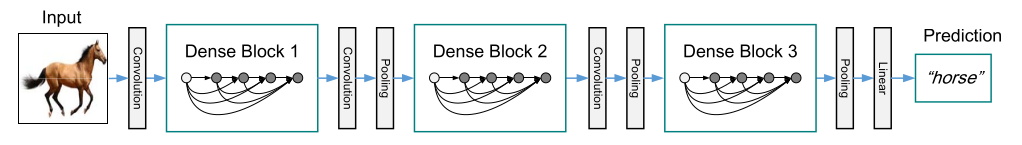
\includegraphics[width=1\textwidth]{img/densenet121_1.png}
    \caption{Una DenseNet profunda con tres bloques densos. Las capas entre dos bloques adyacentes se denominan capas de transición y cambian el tamaño de los mapas de características de
mediante convolución y agrupación \parencite{huang2017densely}.}
    \label{fig:densenet1}
\end{figure}

En conjunto, este enfoque 3D resultó más adecuado para el problema planteado, ya que preserva la información tridimensional completa del pulmón, permitiendo al modelo aprender relaciones espaciales relevantes para la predicción del riesgo de complicaciones tras la biopsia.

\section{Técnicas avanzadas}

\subsection{Pre-entrenamiento en otras tareas similares y fine-tuning}
Uno de los principales desafíos de este proyecto, y en general de muchos trabajos en el ámbito médico, es el tamaño limitado de la base de datos disponible, compuesta en este caso por tan solo 125 pacientes. Este volumen de datos puede resultar insuficiente para entrenar desde cero modelos de deep learning como los descritos anteriormente, ya que puede conducir al sobreajuste o poca generalización.

Para mitigar este problema, se emplea habitualmente una estrategia conocida como \textit{preentrenamiento (pretraining)}, que consiste en entrenar previamente el modelo sobre datos relacionados o tareas similares. De este modo, el modelo parte de un conocimiento inicial que puede facilitar el aprendizaje en la tarea específica y mejorar los resultados finales. Posteriormente, se aplica un \textit{ajuste fino (fine-tuning)}, técnica ampliamente utilizada en aprendizaje profundo para adaptar el conocimiento aprendido en la tarea fuente al dominio objetivo.

El fundamento del preentrenamiento es inicializar el modelo con pesos entrenados previamente en un problema relacionado y con mayor disponibilidad de datos, de forma que la red haya aprendido representaciones generales útiles para la nueva tarea. En este trabajo, se utilizó un conjunto de datos abierto y público, \textit{MedMNIST3D}, que incluye volúmenes de TC asociados a distintas tareas de clasificación anatómica. Aunque las etiquetas de la tarea fuente (órganos o estructuras) no son equivalentes al problema de predicción de complicaciones en biopsias pulmonares, la hipótesis es que el modelo puede aprender características morfológicas y texturales generales del pulmón y otras estructuras corporales que resulten transferibles. Incluso podría captar patrones sutiles que contribuyan a mejorar el rendimiento en nuestro conjunto de datos.

Durante el preentrenamiento se usaron arquitecturas 3D convolucionales (ResNet3D y DenseNet121 3D) entrenadas para tareas de clasificación multiclase en MedMNIST3D. Para obtener el mejor modelo preentrenado, se combinaron diferentes funciones de pérdida, incluyendo \textit{Cross-Entropy}, \textit{Triplet Loss} y \textit{Contrastive Loss} (véase \ref{subsec:pre-contrastivo}), con el objetvo de mejorar la separación entre clases y facilitar su utilidad para transferencia. Todo este entrenamiento se realizó de forma supervisada y con estrategias de data augmentation específicad del dominio 3D.

Una vez finalizado el preentrenamiento, se realizó el ajuste fino (\textit{fine-tuning}) sobre la tarea objetivo: predicción de complicaciones tras biopsia pulmonar. Para ello, se cargaron los pesos preentrenados y se entrenó el modelo en nuestro conjunto de datos. Se evaluaron dos estrategias principales de fine-tuning:

\begin{itemize}
    \item \textbf{Fine-tuning con el backbone congelado:} únicamente se reentrenó la capa de clasificación final. Esta opción tiene la ventaja de evitar el sobreajuste en datasets muy pequeños, limitando el número de parámetros a actualizar.
    \item \textbf{Fine-tuning completo (todo descongelado):} todos los pesos del modelo fueron reentrenados con un learning rate más bajo que en experimentos con modelos sin preentrenar. Esta estrategia permite adaptar mejor las características intermedias del modelo al dominio específico de nuestros volúmenes.
\end{itemize}

Ambas variantes se evaluaron mediante validación cruzada estratificada para medir su capacidad de generalización, comparando métricas como Accuracy, F1-score y G-Mean. 

Si bien en teoría esta técnica debería mejorar el rendimiento, en nuestro caso los modelos preentrenados no lograron superar el rendimiento de los entrenados desde cero (véase el Capítulo \ref{analisis-resultados}). Este resultado puede deberse a que nuestra tarea es muy específica y difiere considerablemente de la tarea fuente. También puede ser que el preentrenamiento haya inducido al modelo a aprender características generales que no resultan suficientemente informativas para nuestro problema concreto.

\subsection{Pre-entrenamiento contrastivo y Deep Metric Learning} \label{subsec:pre-contrastivo}

En la gran mayoría de las implementaciones de estre trabajo hemos utilizado la función de pérdida de entropía cruzada. Incluso en general también son ampliamente utilizadas en muchas aplicaciones de aprendizaje profundo supervisado. Sin embargo, tienden a ser menos adecuados cuando existe una gran varianza intraclase y una baja varianza interclase en la distribución de los datos de entrada. Aquí es cuando surge el concepto de  \textit{Aprendizaje profundo métrico (Deep Metric Learning)} \parencite{mohan2023deep}. El aprendizaje profundo métrico tiene como objetivo que el modelo aprenda a medir la similitud entre muestras al proyectarlas en un espacio de representación donde las relaciones entre clases estén bien estructuradas. En este espacio, las muestras de la misma clase se ubican próximas entre sí, mientras que las de clases diferentes se mantienen separadas. Para lograrlo, se utilizan estrategias de muestreo adecuadas y funciones de pérdida específicas que optimizan la construcción de este espacio, incluso en escenarios donde las clases presentan diferencias sutiles o alta variabilidad interna.

Las dos funciones de pérdida que hemos utilizado en el preentrenamiento han sido \textit{Contrastive Loss} y \textit{Triplet Loss} explicadas matemáticamente en la Sección \ref{sec:contrastive-loss}.

% \subsubsection{Contrastive Loss}

% El objetivo principal de una formulación estándar de \textit{metric learning} es aprender un espacio de representación donde muestras de la misma clase estén cercanas entre sí, mientras que las de clases distintas se mantengan alejadas. Una manera de imponer esta restricción durante el entrenamiento de una red neuronal profunda es mediante la \textit{Contrastive Loss}.  

% Consideremos dos representaciones de características, $f_i$ y $f_j$, asociadas a las muestras $i$ y $j$. Si ambas pertenecen a la misma clase, el objetivo es minimizar la distancia entre sus representaciones. En cambio, si pertenecen a clases distintas, se busca maximizar la distancia al menos hasta un margen $\alpha$. Matemáticamente, la función de pérdida contrastiva se define como:

% \[
% L_{con} = 
% \begin{cases}
% \|f_i - f_j\|^2, & \text{si } y_i = y_j \\
% \left[\alpha - \|f_i - f_j\|^2\right]_+, & \text{si } y_i \neq y_j
% \end{cases}
% \]

% donde $y_i$ y $y_j$ son las clases asociadas a las muestras $i$ y $j$, y $\alpha$ es el margen que determina la distancia mínima deseada entre clases distintas. El operador $[\,\cdot\,]_+$ denota la función \textit{max}($0$, $\cdot$), que asegura no penalizar distancias ya mayores al margen.

% Esta formulación fuerza al modelo a aprender un espacio de características donde las muestras de la misma clase queden agrupadas, mientras que las de diferentes clases se separen al menos una distancia $\alpha$, favoreciendo así la discriminación en el espacio de representación aprendido.

% \vspace{1em}

% \subsubsection{Triplet Loss}

% La \textit{Triplet Loss} es una mejora sobre la formulación de la Contrastive Loss, ampliamente utilizada como objetivo en aprendizaje métrico para crear espacios de incrustación más separables. Esta pérdida considera tres representaciones de características: $f_a$, $f_p$ y $f_n$, correspondientes a una imagen ancla (Anchor), una positiva (Positive) y una negativa (Negative) respectivamente.  

% El par ancla-positiva $(a,p)$ corresponde a dos muestras de la misma clase, mientras que la muestra negativa $n$ pertenece a una clase diferente. El objetivo de la Triplet Loss es minimizar la distancia entre el Anchor y el Positive, al mismo tiempo que se maximiza la distancia entre el Anchor y el Negative, garantizando al menos un margen $\alpha$ de separación.  

% Cuando se utiliza la distancia euclidiana, la formulación de la Triplet Loss es:

% \[
% \mathcal{L} = \sum_{a,p,n \in N} \left[\|f_a - f_p\|^2 - \|f_a - f_n\|^2 + \alpha\right]_+
% \]

% donde $N$ representa el conjunto de todas las tripletas válidas extraídas del conjunto de entrenamiento.  

% Aquí, $\alpha$ define el margen mínimo que se desea imponer entre la distancia Anchor-Negative y la Anchor-Positive.  

% Esta formulación matemática puede entenderse como una extensión de la Contrastive Loss, ya que impone de manera explícita la similitud entre Anchor y Positive mientras repele al Negative. Al aprender a distinguir estas relaciones de tripletas, el modelo construye un espacio de representación más estructurado y discriminativo, adecuado para tareas con alta complejidad intra e interclase.


\subsection{Integración de imágenes médicas y datos clínicos}

En el ámbito del aprendizaje profundo para medicina solemos tener varios tipos de datos, los datos tabulares clínicos de los pacientes y si procede, las imágenes médicas. Por tanto, la integración de ambos tipos de datos puede ser una estrategia prometedora para mejorar la capacidad predictiva de los modelos. En este trabajo, como ya sabemos, tenemos volúmenes de tomografía computarizada que nos proporcionan información anatómica y morfológica detallada del pulmón y datos clínicos tabulares que recogen variables demográficas, antecedentes médicos y factores de riesgo relevantes.  

Combinar estas dos modalidades permite al modelo aprovechar los dos tipos de información: mientras la imagen captura patrones espaciales y texturales, los datos clínicos aportan contexto sobre el estado general del paciente, patologías previas o riesgos. La hipótesis es que integrar ambas fuentes permitirá predecir el riesgo de complicación de forma más precisa que utilizando únicamente una de ellas.  

Para ello, en la implementación se diseñó un modelo híbrido que procesa por separado las dos entradas. Por un lado, el volumen pulmonar segmentado se introduce en una arquitectura DenseNet3D, preprocesada con técnicas de normalización e interpolación para un tamaño uniforme. Esta rama convolucional extrae un conjunto de características profundas (embeddings) que capturan la morfología y textura tridimensional del tejido pulmonar. Por otro lado, los datos clínicos tabulares se introducen en una red neuronal multicapa (MLP, Multilayer Perceptron) con activaciones no lineales y regularización por dropout, que aprende representaciones latentes de las variables clínicas.  

Tras este procesamiento independiente, las salidas de ambas ramas se concatenan en un único vector de características combinadas, que se introduce en una capa fully connected de clasificación binaria. De este modo, el modelo aprende de forma conjunta a combinar la información anatómica extraída de las imágenes con los factores clínicos del paciente, permitiendo capturar interacciones entre ambas fuentes de datos.  

Esta aproximación refleja el enfoque habitual en la práctica clínica, donde los profesionales médicos combinan la información clínica del paciente con la interpretación de las imágenes para tomar decisiones fundamentadas.


\endinput
%--------------------------------------------------------------------
% FIN DEL CAPÍTULO. 
%--------------------------------------------------------------------
